\documentclass[a4paper]{article}

\usepackage{pgfplots}

\usepackage{pgfplotstable}

\begin{document}

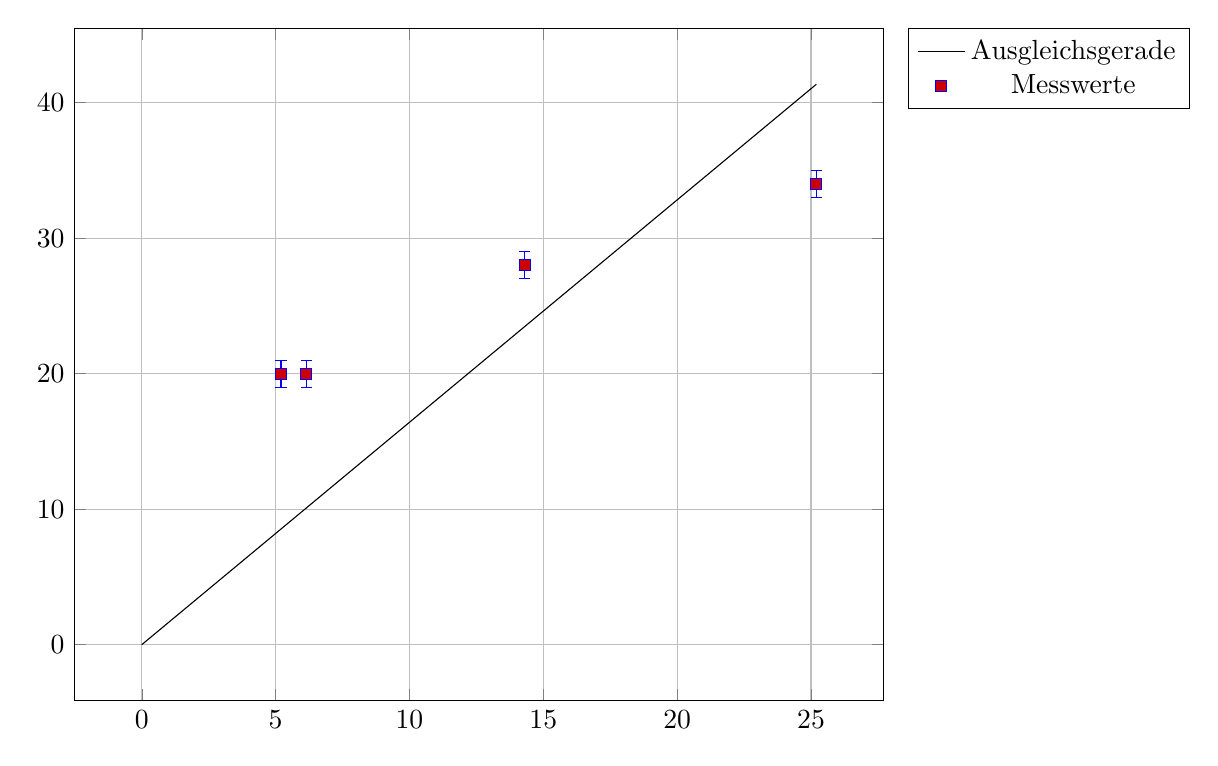
\begin{tikzpicture}
    \begin{axis}[legend pos=outer north east,
      grid=major,
    scale=1.5
    ]
    
		\addplot[no marks] table [
		   y={create col/linear regression={y=Y,variance=V}}]
		   {
		     X  	Y	V
		     0 0 1
		     5.20 20	1000
		     6.14 20	1000
		     14.3 28	1000
		     25.2 34	1000
		     };	
		     \addlegendentry{Ausgleichsgerade}
		     		\addplot+[blue,only marks,error bars/.cd,
			y dir=both,y explicit]
						coordinates {
			(5.20,20) +- (1,1)
			(6.14,20) +- (1,1)
			(14.30,28) 	+- (1,1)
			(25.2,34) +- (1,1)
			};
		\addlegendentry{Messwerte}
    \end{axis}
    
    
  \end{tikzpicture}
\end{document}

